\documentclass[10pt]{article}
\usepackage{tkz-euclide}
\usetkzobj{all}
\usetikzlibrary{arrows.meta}
\usepackage[title]{appendix}
\usepackage{amssymb}
\usepackage{amsmath}
\usepackage{tikz}
\usepackage[autolinebreaks, framed]{mcode}
\usepackage{graphicx}
\usepackage{verbatim}
\usetikzlibrary{patterns}
\usepackage[margin=1.4in]{geometry}
\usepackage{graphicx}

\usepackage{verbatimbox}
\newcommand{\inlinemaketitle}{{\let\newpage\relax\maketitle}}

\title{PSBC Project 2}
\begin{document}

\inlinemaketitle
\section{Introduction}

This report details the approach and implementation relating to the second coursework project of MATH36032. Please note that all programming and testing was carried out using GNU Octave rather than MATLAB.

\section{The Problem}

The goal of this project is to investigate the dynamics between a fox and a rabbit in a specific scene. The goal of the rabbit in the scene is to reach it is a burrow safely. Meanwhile, the goal of the fox is to catch the rabbit. We will aim to answer the question of which outcome occurs based on a set of input parameters.

To do this, we will use differential equations, solving them numerically using Octave's \texttt{ode45} solver.

\section{The Scene}

The scene we will be working with is as follows. Its main feature is a warehouse defined by its two westerly corners which we will denote as $NW$ and $SW$ for northwest and southwest respectively. The scene will contain the rabbit's burrow (denoted $B$). Figure \ref{fig:scene} shows an example configuration. We will denote the position of the rabbit by $R$ and the fox by $F$.

The rabbit moves in a straightforward way, directly towards the burrow with constant speed $s_{r0}$. The fox moves under the following rules.

\begin{equation}
\label{lbl:movementRules}
\begin{array}{p{0.9\textwidth}}
\begin{itemize}

\item If the rabbit is within the fox's line of sight, the fox runs directly towards the rabbit.

\item If a corner of the warehouse obscures the rabbit, then the fox runs towards that corner.

\item If the fox reaches a corner and the rabbit still is not in sight, it follows the warehouse perimeter until it sees the rabbit.
\end{itemize}
  \end{array}
\end{equation}

Before continuing, we must make a few assumptions as to what our model can support. They are as follows.

\begin{itemize}

\item The rabbit is within the fox's line of sight initially.
\item The burrow is within the rabbit's line of sight initially.

\end{itemize}

\section{The General Approach}

The approach we will use is to model the scene using Octave's built-in \texttt{ode45} function, which is a numerical solver for ODEs. We will take advantage of the fact that it is a numerical solver, not a symbolic one, allowing us will allow us to change the direction of the fox within the ODE function. These changes are based on the fox's line of sight, and the other factors referenced in the rules above. 

We can do this because of the iterative nature of the solver, meaning that changing the target will not affect the values computed for previous timeframes.

\section {The Solution}

The first two inputs to our function defining the ODE are time $t$, and the vector $z$ holding the solution at $t$, this is defined by

\begin{align}
    z &= \begin{bmatrix}
           R_x \\
           R_y \\
           F_x \\
           F_y
         \end{bmatrix}.
  \end{align}

Within our ODE function, we must calculate the derivative of the elements of $z$ with respect to time. 

\begin{align}
    \dot{z} &= \begin{bmatrix}
            \dot{R_x} \\
            \dot{R_y} \\
            \dot{F_x} \\
            \dot{F_y}
         \end{bmatrix}.
  \end{align}
 
In other words, we will calculate the velocity of the fox and rabbit in the $x$ and $y$ directions at time $t$.

We will break the problem up into smaller pieces and solve these small pieces first before looking at the solution as a whole. In practice, this means examining small helper functions which will contribute to the final solution.

\subsection {Determining the Fox's Target} \label{lbl:foxtarget}

The most challenging aspect of modeling this scene is to determine the direction in which the fox should run at any instant, following \ref{lbl:movementRules}. We will solve this problem by splitting our scene up into three overlapping regions $A$, $B$ and $C$ defined as follows (and visualized in \ref{fig:zones}). 

$$ A = \{ (x,y) \in \mathbb{R}^2  \mid  y > NW_y \},  $$
$$ B = \{ (x,y) \in \mathbb{R}^2  \mid  x < NW_x \},  $$
$$ C = \{ (x,y) \in \mathbb{R}^2  \mid  y < SW_y \}.  $$

\begin{figure}
\caption{The scene divided into three regions}
\centering
\label{fig:zones}
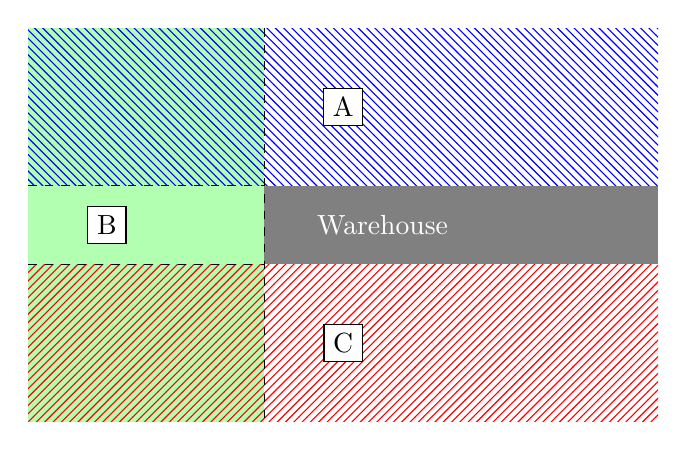
\begin{tikzpicture}  


\fill (0,1) [fill=green, fill opacity=0.3] rectangle (3,6);
\fill (0,4) [pattern=north west lines, pattern color=blue] rectangle (8,6);
\fill (0,1) [pattern=north east lines, pattern color=red] rectangle (8,3);

\fill (3,3) [gray] rectangle (8,4);
\draw [dashed] (0,3) -- (3,3);
\draw [dashed] (0,4) -- (3,4);
\draw [dashed] (3,6) -- (3,1);

\node[draw, fill=white] at (4,5) {A};
\node[draw, fill=white] at (1,3.5) {B};
\node[draw, fill=white] at (4,2) {C};

\node[text=white, draw=gray] at (4.5,3.5) {Warehouse};

\end{tikzpicture}
\end{figure}

The rules dictate that the fox always runs towards something, either the rabbit or one of the corners. We refer to this as the fox's target.

Cleary, if both the fox and rabbit are in the same zone, then the fox's target is the rabbit since there must be a line of sight between them. 

Now suppose this is not the case and the fox and the rabbit are in different zones. Let $L$ denote the line connecting the fox and the rabbit, and it's equation be $y = mx  + c$. We check if this line intersects the south wall of the warehouse or the west wall of the warehouse. Note, since the warehouse in convex, there is no need to check intersection with the north wall. Since if there is an intersection with the north wall, then there must be an intersection with one of the other two.

Before continuing, a note on why we first excluded the case where both creatures are in the same zone. The reason is that $L$ could intersect one or both of the walls, but the fox still has a line of sight. This happens only when they are in the same zone. Excluding this case first makes for easier calculations since we can then assume that an intersection means there is no line of sight.

Let $\Delta_x$, $\Delta_y$ denote the horizontal and vertical distances respectively between the fox, and the target. The gradient $m$ therefore is $\frac{\Delta_y}{\Delta_x}$. In the equation above $c$ is referred to as the intercept (the $y$ coordinate when $x = 0$). This is calculated $c = F_y - m \times F_x$. \\

\noindent \textbf{West wall}

To check if $L$ intersects the west wall, we must calculate the $y$ coordinate of $L$ at $x = SW_x$. If this value lies between $SW_y$ and $NW_y$ then we have an intersection. Mathematically, we check if the following holds.

$$ SW_y < m \times SW_x + c < NW_y.$$\\

\noindent \textbf{South wall}

Intersection with the south wall happens if the $x$ coordinate where $L$ intersects the line $y = SW_y$ is strictly greater than $SW_x$. By rearranging the equation of $L$, we see that we have intersection when the following holds.

$$ \frac{SW_y - c}{m} > SW_x. $$

We can conclude that if either case holds then the fox doesn't have a line of sight to the rabbit and hence the rabbit cannot be the fox's target. Leaving the northwest corner and southwest corner of the warehouse the only two possibilities.

If the fox is in zone $A$, then the target is $NW$ clearly, since the closest corner to the fox is $NW$. Similarly, if the fox is in zone $C$ then the target must be $SW$. 

The final case is when the fox is in zone $B$ but \emph{not} in zones $A$ or $C$. In this case, the fox's target depends on the location of the rabbit. If the rabbit is in zone $A$ then the target is $NW$, otherwise, the target is $SW$. A simple way to check this is to consider whether the gradient $m$ is positive or negative. If it's positive then the rabbit must be in zone $A$ and if negative it must be in zone $C$.

This also accounts for the rule that states that the fox follows the perimeter if it is at one of the corners but can't see the rabbit. Let's look at the case where the fox is at $NW$ and can't see the rabbit, then it must be the case that the rabbit is southeast of the warehouse, making the gradient negative, meaning the fox target will be $SW$.

Conversely, if the fox is at $SW$ and can't see the rabbit, then it is north of $SW$ and $m$ must be positive since the rabbit must be northeast of the warehouse.

The implementation of this function is listed in Listing \ref{lst:computeFoxTarget}. The first two lines of this function demand some explanation. They define variables \texttt{X} and \texttt{Y} to use when indexing the vectors. The reasoning is as follows. Given a vector \texttt{a = [xComponent, yComponent]}, it is far more readable to write code using \texttt{a(X)} and \texttt{a(Y)}, than \texttt{a(1)} and \texttt{a(2)}.

 \lstinputlisting[label={lst:computeFoxTarget}, caption={A function to compute the fox's target given the warehouse coordinates and the rabbit's position.}] {../computeFoxTarget.m}

\subsection {Velocities in the $x$ and $y$ directions}

We've seen in part \ref{lbl:foxtarget} that the fox always runs towards some target with constant speed. Furthermore, the rabbit perpetually runs towards its burrow, also with constant speed. Therefore, we can say that a creature $C$ runs towards a target $T$ with a constant speed of $u$. We seek it's velocity in the $x$ direction ($v_x$) and in the $y$ direction ($v_y$).



\begin{figure}[h]
\label{fig:chasing}
\caption{The scenario when a creature C runs towards a target T.}
\centering
\begin{tikzpicture}
 
\coordinate (O) at (-1,0);
\coordinate (A) at (3,0);
\coordinate (B) at (3,2);
\draw[dashed] (O)--(A);
\draw[dashed] (A)--(B);
\draw[-{Latex[width=2mm]}] (O)--(B);

\filldraw (-1,0) circle[radius=1.5pt];
\node[above left=0pt of {(-1,0)}, outer sep=1pt,fill=white] {C};

\filldraw (3,2) circle[radius=1.5pt];
\node[above right=0pt of {(3,2)}, outer sep=1pt,fill=white] {T};


\tkzLabelSegment[below=1pt](O,A){$\Delta_x$}
\tkzLabelSegment[above=2pt](O,B){$\Delta$}
\tkzLabelSegment[right=2pt](A,B){$\Delta_y$}

\tkzMarkRightAngle[size=0.5,opacity=.4](O,A,B)% square angle here

\tkzLabelAngle[pos = 0.85](B,O,A){$\theta$}
\tkzMarkAngle[fill=gray, size=1.2cm, opacity=.4](A,O,B)


\end{tikzpicture}
\end{figure}


Figure \ref{fig:chasing} shows the scene. Using this we denote the angle between the creature and the target by $\theta$ and the distance between them by $\Delta$. We can then easily deduce that

$$ v_x = u\cos{\theta}, $$
$$ v_y = u\sin{\theta}. $$

Furthermore, we see there's no need to compute $\theta$. We can observe that 

$$ \cos{\theta} = \frac{\Delta_x}{\Delta}$$
$$ \sin{\theta} = \frac{\Delta_y}{\Delta}.$$

We can then combine these equations giving our final equations

$$ v_x = u \frac{\Delta_x}{\Delta},$$
$$ v_y = u \frac{\Delta_y}{\Delta}.$$

The advantage of using these equations rather than computing $\theta$ using trigonometry is that we can implement both components in one line using Octave's vector based arithmetic. We can see this in our implementation in Listing \ref{lst:computeVelocity}.

Note, this function calls a function called \texttt{distance}, which simply computes the distance between two points. It is listed as Listing \ref{lst:distance} in Apprendix \ref{ap:distance}.

 \lstinputlisting[label={lst:computeVelocity}, caption={A function to compute the velocity of an entity facing a target with a given speed.}] {../computeVelocity.m}


\subsection {Stopping the ODE solver}

We can use an event function to stop the computation when our one of our end conditions is satisfied. Two events should stop the calculation, the fox catching the rabbit, and the rabbit reaching the burrow.

We will use a similar approach for both. The rabbit is considered caught if it is within 0.1 meters of the fox. Similarly, it is deemed to be in its burrow if it is within 0.1 meters of it. \emph{Note} that this could present an issue in situations where the fox is very close to the rabbit at the same time as the rabbit is very close to the burrow. It could be ambiguous whether the rabbit is safe or not. In these cases, it may be appropriate to choose a smaller value than 0.1 to ensure the correct result is output.

Let the distance between the fox and the rabbit be $\Delta_{f,r}$. Our event function should trigger the ODE solver to stop when $\Delta_{f,r}$ becomes less than 0.1. In other words when $\Delta_{f,r} - 0.1$ becomes negative. The case when the rabbit reaches the burrow is similar. The implementation is listed in Listing \ref{lst:stopEvent}.

 \lstinputlisting[label={lst:stopEvent}, caption={The event function used to stop the ODE solver.}] {../stopEvent.m}



With this in place, we can now examine the ODE function itself, included in Listing: \ref{lst:modelode}. We can see that we compute the rabbit's velocity directly, and compute the fox's velocity based on its trajectory.

 \lstinputlisting[label={lst:modelode}, caption={The ODE function used to model the fox chasing the rabbit}] {../modelODE.m}







\section{A more realistic scenario}
\section{A more realistic scenario}

\begin{appendices}

\section{Distance}\label{ap:distance}
 \lstinputlisting[label={lst:distance}, caption={A function to compute the distance between two points.}] {../distance.m}


\section{The \texttt{plotScene} function}\label{ap:plotScene}
 \lstinputlisting[label={lst:plotScene}, caption={A function to plot the results of the ODE solver and the rest of the scene.}] {../plotScene.m}
\end{appendices}


\begin{thebibliography}{9}
\end{thebibliography}

\end{document}
